\documentclass[preprint, 3p,
authoryear]{elsarticle} %review=doublespace preprint=single 5p=2 column
%%% Begin My package additions %%%%%%%%%%%%%%%%%%%

\usepackage[hyphens]{url}

  \journal{Astronomy and Computing} % Sets Journal name

\usepackage{lineno} % add

\usepackage{graphicx}
%%%%%%%%%%%%%%%% end my additions to header

\usepackage[T1]{fontenc}
\usepackage{lmodern}
\usepackage{amssymb,amsmath}
\usepackage{ifxetex,ifluatex}
\usepackage{fixltx2e} % provides \textsubscript
% use upquote if available, for straight quotes in verbatim environments
\IfFileExists{upquote.sty}{\usepackage{upquote}}{}
\ifnum 0\ifxetex 1\fi\ifluatex 1\fi=0 % if pdftex
  \usepackage[utf8]{inputenc}
\else % if luatex or xelatex
  \usepackage{fontspec}
  \ifxetex
    \usepackage{xltxtra,xunicode}
  \fi
  \defaultfontfeatures{Mapping=tex-text,Scale=MatchLowercase}
  \newcommand{\euro}{€}
\fi
% use microtype if available
\IfFileExists{microtype.sty}{\usepackage{microtype}}{}
\usepackage[]{natbib}
\bibliographystyle{plainnat}

\ifxetex
  \usepackage[setpagesize=false, % page size defined by xetex
              unicode=false, % unicode breaks when used with xetex
              xetex]{hyperref}
\else
  \usepackage[unicode=true]{hyperref}
\fi
\hypersetup{breaklinks=true,
            bookmarks=true,
            pdfauthor={},
            pdftitle={Using Machine Learning to Predict the Correlation of Spectra Using SDSS Colour Magnitudes as an Improvement to the Locus Algorithm},
            colorlinks=false,
            urlcolor=blue,
            linkcolor=magenta,
            pdfborder={0 0 0}}

\setcounter{secnumdepth}{5}
% Pandoc toggle for numbering sections (defaults to be off)


% tightlist command for lists without linebreak
\providecommand{\tightlist}{%
  \setlength{\itemsep}{0pt}\setlength{\parskip}{0pt}}






\begin{document}


\begin{frontmatter}

  \title{Using Machine Learning to Predict the Correlation of Spectra
Using SDSS Colour Magnitudes as an Improvement to the Locus Algorithm}
    \author[Technological University Dublin]{Tom O'Flynn}
   \ead{tom.oflynn@tudublin.ie} 
    \author[Technological University Dublin]{Eugene Hickey%
  %
  \fnref{1}}
   \ead{eugene.hickey@tudublin.ie} 
    \author[Technological University Dublin]{Kevin Nolan%
  %
  \fnref{2}}
   \ead{kevin.nolan@tudublin.ie} 
    \author[Dublin Institute of Advanced Studies]{Oisin Creaner%
  %
  \fnref{2}}
   \ead{creanero@cp.dias.ie} 
      \affiliation[Technological University Dublin]{Department of
Applied Science, Technological University Dublin D24FKT9, Ireland.}
    \affiliation[Dublin Institute of Advanced Studies]{Dublin Institute
of Advanced Studies, 10 Burlington Rd, Dublin, D04 C932, Ireland}
    \cortext[cor1]{Corresponding author}
    \fntext[1]{Corresponding Author}
    \fntext[2]{Equal contribution}
  
  \begin{abstract}
  The Locus Algorithm is a new technique to improve the quality of
  differential photometry by optimising the choices of reference stars.
  At the heart of this algorithm is a routine to assess how good each
  potential reference star is by comparing its sdss magnitude values to
  those of the target star. In this way, the difference in
  wavelength-dependent effects of the Earth's atmospheric scattering
  between target and reference can be minimised. This paper sets out a
  new way to calculate the quality of each reference star using machine
  learning. A random subset of stars from sdss with spectra was chosen.
  For each one, a suitable reference star, also with a spectrum, was
  chosen. The correlation between the two spectra was taken to be the
  gold-standard measure of how well they match up for differential
  photometry. The five sdss magnitude values for each of these stars
  were used as predictors. A number of supervised machine learning
  models were constructed on a training set of the stars and were each
  evaluated on a testing set. The model using Support Vector Regression
  had the best performance of these models. It was then tested of a
  final, hold-out, validation set of stars to get an unbiased measure of
  its performance. The dataset used, the model constructions, and
  performance evaluation are presented here.
  \end{abstract}
  
 \end{frontmatter}

\hypertarget{introduction}{%
\section{Introduction}\label{introduction}}

A wealth of astrophysics information is available through the study of
the brightness of celestial objects as a function of time. For example,
exoplanet detection by the transit method relies critically on
measurements of intrinsic variability where such variability can be a
small fraction of the total stellar brightness (\citet{Giltinan2011},
\citet{Everett2001}). Ground-based observations looking for such
variability are complicated by the effects of the Earth's atmosphere
which causes incoherent wavelength-dependent variations in the stellar
flux detected. This can mask intrinsic variability and hamper the study
of variable astrophysical phenomena (\citet{Smith2008}).

The technique of differential photometry has been developed in an
attempt to mitigate the effects of the Earth's atmosphere on studies of
stellar variability. Differential photometry uses references stars at
small angular separations from the star of interest as comparators.
Atmospheric effects should have similar effects on the measured flux
from all of these stars causing them to vary in unison
(\citet{Burdanov2014}). Because scattering in the Earth's atmosphere is
wavelength dependent, the technique is especially successful if the
target star and reference stars are spectrally similar
(\citet{Milone2011a}, \citet{Sterken2011}).

The Locus Algorithm (\citet{creaner2022}) has been used to create
catalogues of pointings suitable for differential photometry on
astromonical targets based on a novel technique of choosing appropriate
reference stars (\citet{creaner2020} and Creaner EXO's). The algorithm
no longer places the target in the centre of the field of view but, in
general, repositions it so as to include the best set of reference
stars. Assessment of each reference star is performed by referring to
the sdss catalogue and the colour band magnitudes therein. These
magnitudes can be used to infer the overall shape of the star's
spectrum. Stars that have similar spectra will be effected by scattering
from the Earth's atmosphere to a more comparable degree that stars with
dissimilar spectra. The original Locus Algorithm used a rational, but
ad-hoc, method to estimate the correlation of stellar spectra based on
differences between their g, r, and i sdss colour magnitudes
(\citet{Creaner2017}). This was necessary for computational efficiency.
The work presented here presents a more rigorous technique to estimate
the correlation of stellar spectra based on machine learning. The subset
of stars in sdss that have their spectra measured are used. These stars
are paired off such that each pair has similar colour magnitude
differences and are thus potentially a good match for differential
photometry. This corresponds to the pre-filtering step employed by
\citet{Creaner2017}. The correlation between each pair's spectra is
calculated. This forms the basis of a goodness-of-fit between the two
spectra. The sdss magnitudes (u, g, r, i, and z for both stars in the
pair) are then used to train machine learning algorithms to predict this
goodness-of-fit. The models produced are then applied to other pairs of
stars, the test set, to evaluate their performance. The results show a
significant improvement over the original ad-hoc Locus Algorithm
routine, this model will be incorporated to future generations of the
Locus Algorithm.

\hypertarget{data}{%
\section{Data}\label{data}}

This work uses 3556 stellar spectra from the SDSS SEGUE and BOSS
observations and their physical parameters from the \(13^{th}\) SDSS
data release (\citet{Aguado2018}). The spectra are clipped to just the
wavelengths contained in the sdss r band (between 550nm and 700nm).
Stars are paired off based on their sdss colour magnitudes so that both
stars in a pair are of similar colour. Specifically, both
\((g_1-r_1)-(g_2-r_2)\) and \((r_1-i_1)-(r_2-i_2)\) will be between 0
and 0.3. This ensures that these stars would be realistic matches for
differential photometry. In addition, stars were chosen that had r
colour magnitude values between 15 and 20. The SQL queries used to
download physical parameters and the spectra are given in the
supplementary materials for this paper. Correlations between spectra are
calculated using the usual Pearson Correlation formula, equation
(\ref{eq:correlation}).

\begin{equation}
  \displaystyle r_{xy}={\frac {n\sum x_{i}y_{i}-\sum x_{i}\sum y_{i}}{{\sqrt {n\sum x_{i}^{2}-\left(\sum x_{i}\right)^{2}}}~{\sqrt {n\sum y_{i}^{2}-\left(\sum y_{i}\right)^{2}}}}}.
  \label{eq:correlation}
\end{equation}

where \(x_i\) refer to the flux from the first star at a given
wavelength, \(i\), in units of \(erg/cm^2/s Å\), \(y_i\) refer to the
flux from the second star at the same wavelength. Figure
\ref{fig:spectra} shows some pairs of stars along with their
correlations. The first pair, A and B, are representative of the sample.
The second pair, C and D, were chosen to have an unusually low
correlation for this sample set.

\begin{figure}
  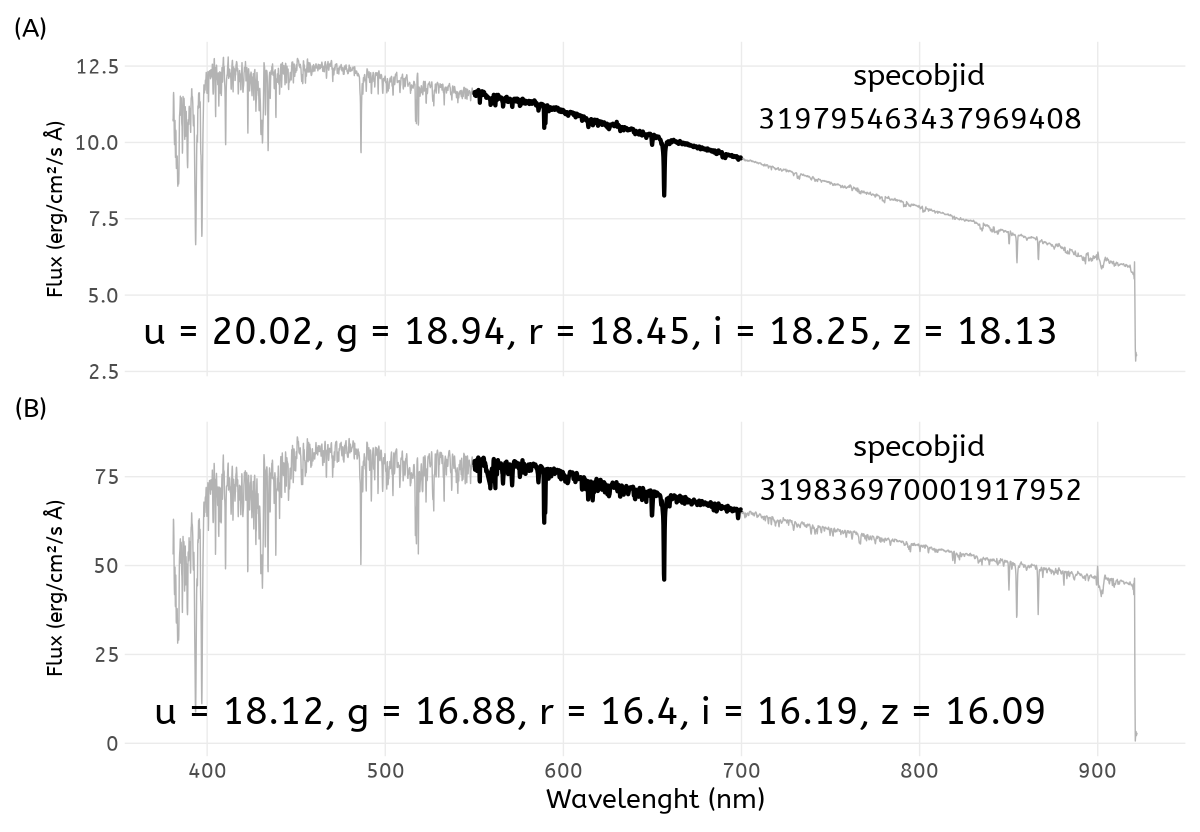
\includegraphics[width=\columnwidth, height = 8cm]{figures/spectra1}
  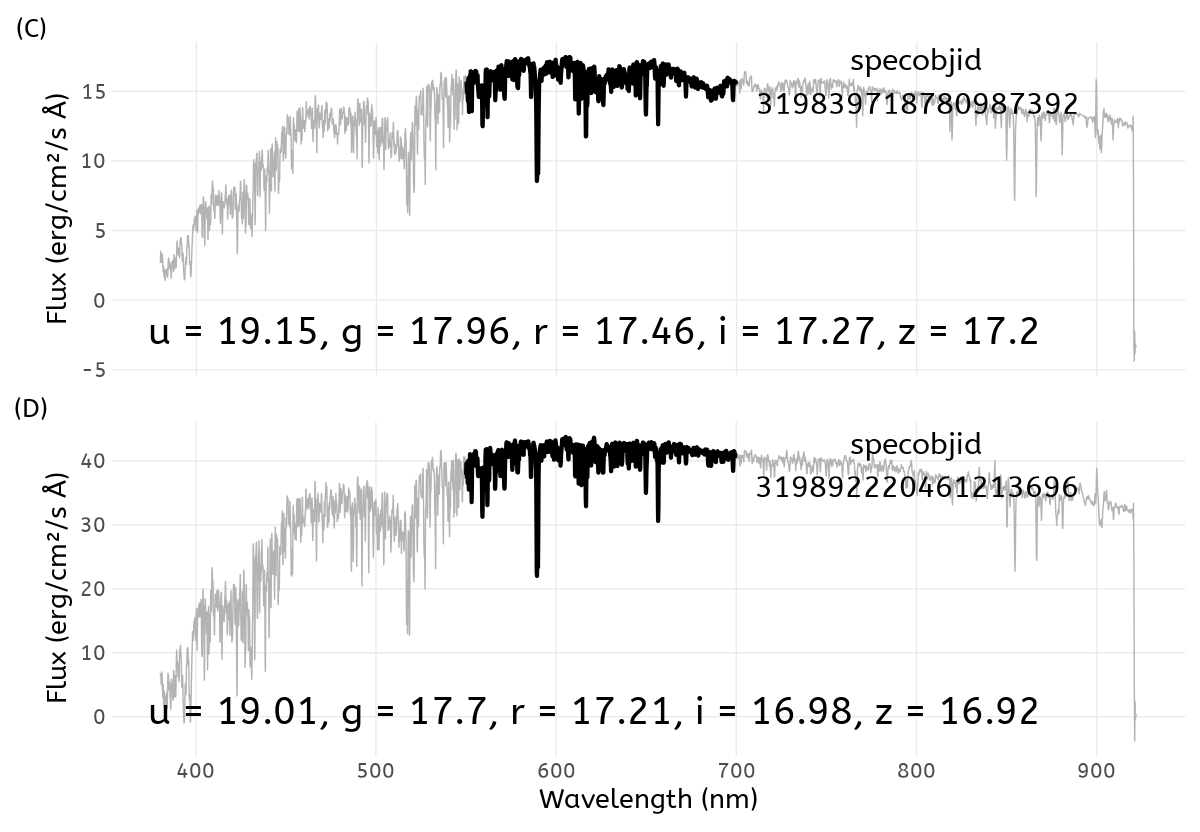
\includegraphics[width=\columnwidth, height = 8cm]{figures/spectra2}
    \caption{Two pairs of spectra downloaded from SDSS. The ugriz colour magnitudes for each star is given below its spectrum. The darkened area of the spectral line corresponds to the r-band wavelengths. The correlation between spectra A and C is 0.96. That between spectra B and D is 0.75.}
    \label{fig:spectra}
\end{figure}

Correlation is usually bounded by -1 and 1. And because these are
spectra from stars and they have similar colour magnitudes, the
correlations tend to be clustered near this higher end, see the
histogram in figure \ref{fig:histograms}A below. Machine learning
algorithms work better with normally distributed values (need reference)
and this is especially true when it comes to analysing model performance
(another reference), so the correlation values were transformed. First
of all by a logit transformation (\ref{eq:logit}):

\begin{equation}
  \displaystyle \operatorname {logit} (x)=\ln \left({\frac {1+x}{1-x}}\right)
  \label{eq:logit}
\end{equation}

And then by scaling and normalising the values to have a mean of 0 and a
standard deviation of 1. The resulting transformed values are shown in
figure \ref{fig:histograms}B.

\begin{figure}
  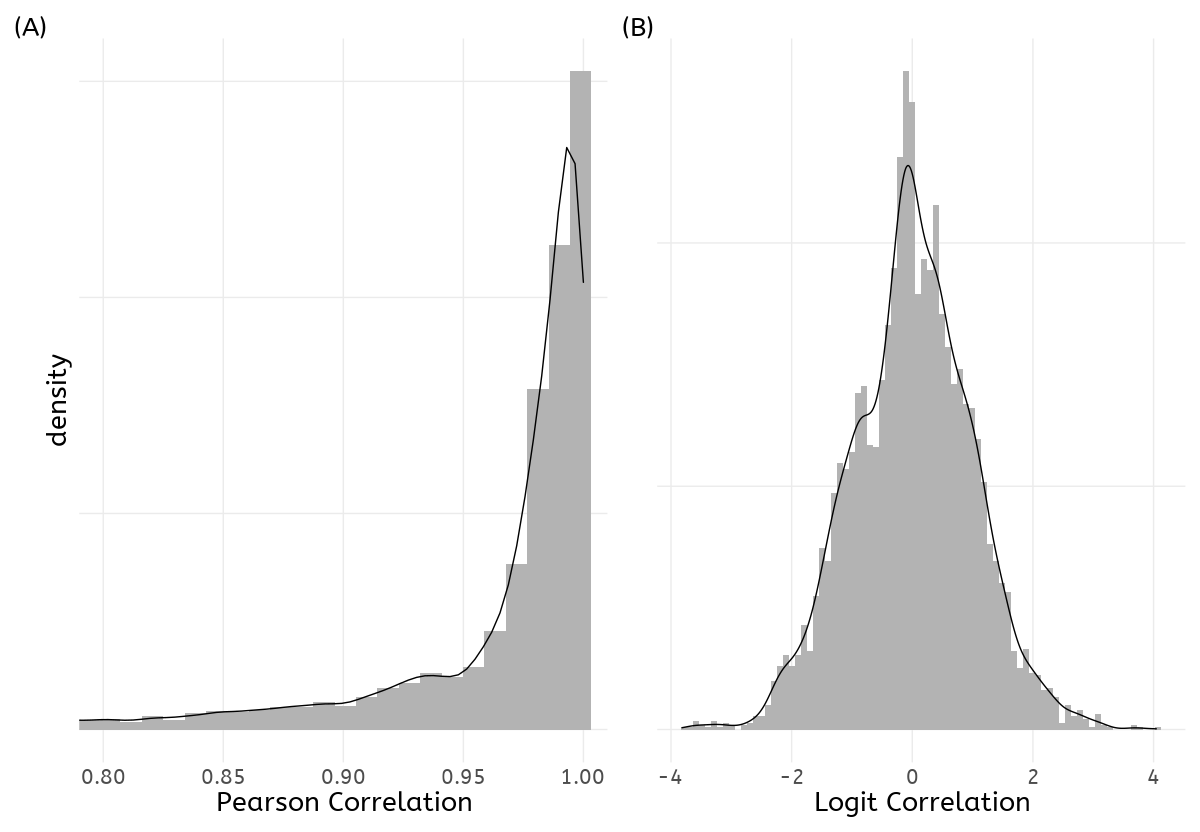
\includegraphics[width=\columnwidth, height = 5cm]{figures/histograms}
    \caption{(A) Histogram of Pearson correlation values between r-band spectra between pairs of matched stars. (B) Values in (A) transformed by a logit function.}
    \label{fig:histograms}
\end{figure}

The data is split into test and training sets, with 70\% of the data
(2668 samples) in the training set and the remainder (888 samples) in
the test set. Each set has a representative sample of correlation
values, to do this the original sample of 3556 pairs is split into five
groups based on percentiles of the correlation and both testing and
training sets get a commensurate proportion of each group. In
additional, completely independent set of 526 pairs of stars are used
for final validation of the chosen model.

\hypertarget{models}{%
\section{Models}\label{models}}

Four types of machine learning algorithms were used: support vector
regression (SVR), random forrest (RF), gradient boosting (GBM), and a
linear model (LM). In each of the four cases, a model was built on the
training set, using 10 predictors, namely the ugriz values for both
stars in each pair. The target value was the logit(correlation) value.
Cross validation, 20-fold repeated 10 times, was used to minimise model
bias. Hyperparameters for each model were tuned. The results for RMSE,
MAE, and \(R^2\) for all models are given in table \ref{tbl:models}.The
details are given below:

\begin{itemize}
\item
  \emph{Support Vector Regression} This used a radial basis kernal
  function (Karatzoglou2004). A grid search on the hyperparameters Cost
  (C) and sigma (\(\sigma\)) was undertaken for values 8 \textless{} C
  \textless{} 25 and 0.08 \textless{} \(\sigma\) \textless{} 0.20. The
  model was optimised based on the RMSE of the training set. The best
  tune was obtained for C = 20 and \(\sigma\) = 0.12.
\item
  \emph{Stochastic Gradient Boosting} This used Friedman's gradient
  boosting algorithm (\citet{Boehmke2019}). A grid search on the
  hyperparameters Number of Boosting Iterations (n.trees), Maximum Tree
  Depth (interaction.depth), Shrinkage (shrinkage), and Minimum Terminal
  Node Size (n.minobsinnode) was undertaken. The model was optimised
  based on the RMSE of the training set. The best tune was obtained for
  n.trees = 100, interaction.depth = 10, shrinkage = 0.1 and
  n.minobsinnode = 10.
\item
  \emph{Random Forrest} This used the \emph{ranger} fast implementation
  of random forrests (\citet{Wright2017}). The Minimum Node Size was set
  to be 5, the splitting rule was chosen to be \emph{variance}. The
  number of variables to possibly split at each node (mtry) was tuned to
  be 6.
\item
  \emph{Linear Model} The final model was a linear model from the MASS R
  package (\citet{Venables2002}). There were no tunable parameters.
\end{itemize}

\hypertarget{model-evaluation}{%
\section{Model Evaluation}\label{model-evaluation}}

The table below gives the values for RMSE, MAE, and \(R^2\) for each of
the four values as they applied to the test set of 888 stellar pairs.

\begin{table}
  \centering
  \caption{Results of applying the best tuned models on the test set. Root mean squared error (RMSE), R-squared value (R2), and mean average error (MAE) for each of the four model types. The models were built on the training set of 2668 stellar pairs. The values given below were obtained by applying each model to the test set of 888 stellar pairs}
  \label{tbl:models}
  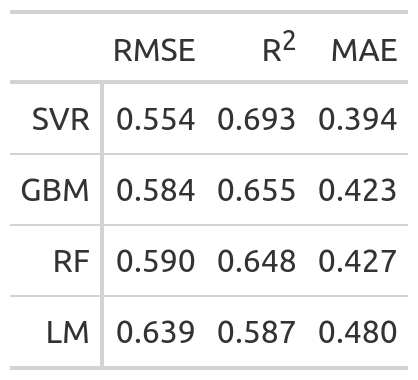
\includegraphics[width=6cm]{figures/model-values-test}
\end{table}

As can be seen from table \ref{tbl:models}, the best performing model
was that produced by SVR. This is in line with expectations as our data
set had few (10) predictors, they were all numeric as opposed to being a
mix of numeric and categorical, and there were no missing values. These
are all factors that favour SVR models.

Finally, the SVR model was applied to the validation set of 526 stellar
pairs. The resulting predicted values has an RMSE of 0.564, an \(R^2\)
of 0.682, and an MAE of 0.399 when compared to the observed logit
correlation values of the spectra. To put these RMSE and MAE values on
context, remember that the logit correlation values have been scaled to
have a standard deviation of 1.

The histogram of the residuals from this fit is shown in figure
\ref{fig:histogram-residuals}. Figure \ref{fig:obs-pred} shows the
resulting values of observed logit correlation values against predicted
logit correlation values. Figure \ref{fig:residuals-pred} shows the
resulting values of the residuals, the observations minus the predicted
values, against predicted logit correlation values. Figure
\ref{fig:residuals-qq} shows a quantile-quantile (QQ) plot of the
residuals.

\begin{figure}
  \centering
  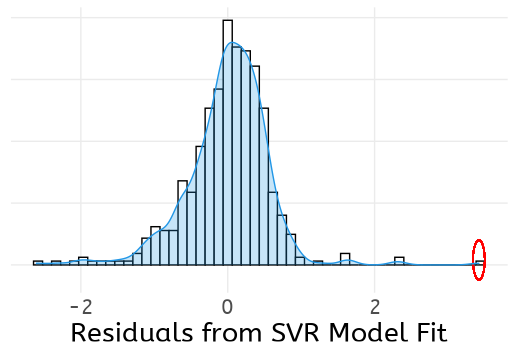
\includegraphics[width=\columnwidth, height = 5cm, width = 10cm]{figures/histogram}
    \caption{Residuals from the fit of the best performing SVR model on the validation dataset. Note one of the outlying values circled in red}
    \label{fig:histogram-residuals}
\end{figure}

All of these plots point to the presence of outliers in the residuals.
These were investigated. Looking at the histogram in figure
\ref{fig:histogram-residuals}, there is a notable residual at 2.3,
highlighted in red in the figure. The spectra of the pair of stars
involved in this outlier were investigated and are shown in figure
\ref{fig:outlier-spectra}. Note that the top spectrum, from a star of
spectral subclass CV located at \(RA = 140.04^{\circ}\) and
\(Dec = 0.7125^{\circ}\), has emission lines rather than absorption
lines more reminiscent of a galaxy rather than a star. This behaviour
was noted for some, but not all, of the stellar pairs with high
residuals. In all cases it involved a star with subclass CV.

\begin{figure}
\centering
  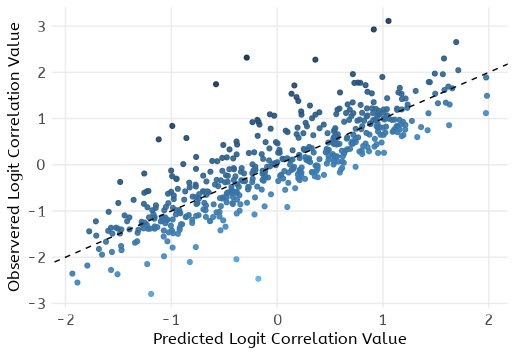
\includegraphics[width=\columnwidth, height = 6.5cm, width = 10cm]{figures/observed-predicted}
    \caption{Observed versus predicted logit correlation values}
    \label{fig:obs-pred}
\end{figure}

\begin{figure}
\centering
  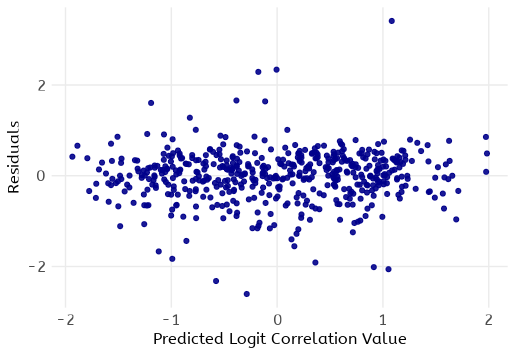
\includegraphics[width=\columnwidth, height = 6.5cm, width = 10cm]{figures/residuals-predicted}
    \caption{Residuals versus predicted logit correlation values}
    \label{fig:residuals-pred}
\end{figure}

\begin{figure}
\centering
  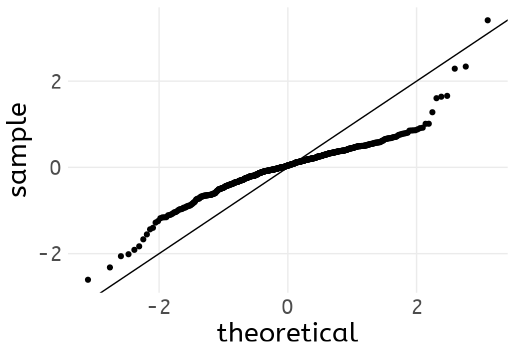
\includegraphics[width=\columnwidth, height = 6.5cm, width = 10cm]{figures/residuals-qq}
    \caption{QQ Plot of the Residuals from the Fit of the SVR Model on the Validation Dataset}
    \label{fig:residuals-qq}
\end{figure}

\begin{figure}
  \centering
  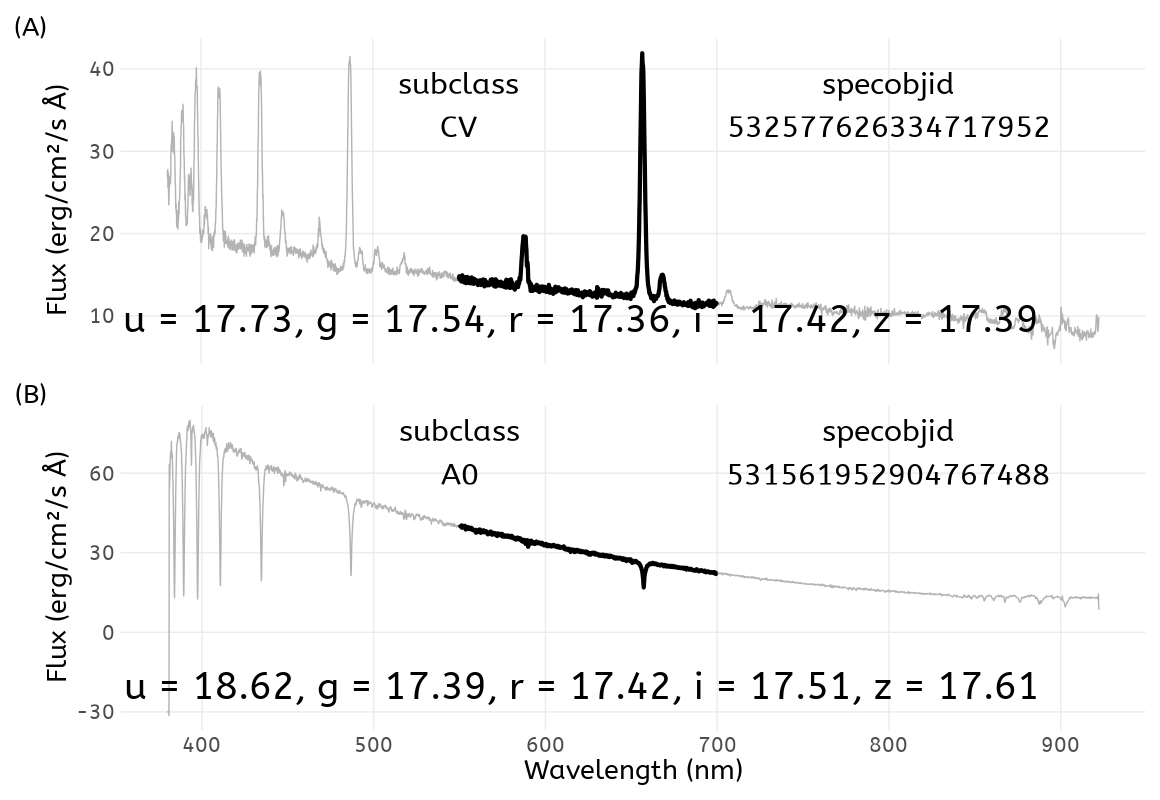
\includegraphics[width=\columnwidth, height = 10cm, width = 10cm]{figures/outlier-spectra}
    \caption{Spectra of the two stars involved in the outlier of the residuals histogram}
    \label{fig:outlier-spectra}
\end{figure}

\hypertarget{conclusions}{%
\section{Conclusions}\label{conclusions}}

The last numbered section should briefly summarise what has been done,
and describe the final conclusions which the authors draw from their
work.

\renewcommand\refname{References}
\bibliography{SDSS.bib}


\end{document}
